%% AgriVision — IEEE conference paper (IEEEtran, two-column)
%%
%% Compile with:  pdflatex agrivision_ieee.tex   (run twice for references)
%% Requires: IEEEtran, graphicx, amsmath, amssymb, booktabs, tikz, pgfplots, url
%% All of these ship with TeX Live, MiKTeX and Overleaf.

\documentclass[conference]{IEEEtran}
\IEEEoverridecommandlockouts

\usepackage{cite}
\usepackage{amsmath,amssymb,amsfonts}
\usepackage{graphicx}
\usepackage{textcomp}
\usepackage{xcolor}
\usepackage{booktabs}
\usepackage{url}
\usepackage{tikz}
\usepackage{pgfplots}
\pgfplotsset{compat=1.17}
\usetikzlibrary{arrows.meta,positioning,fit,backgrounds}

\def\BibTeX{{\rm B\kern-.05em{\sc i\kern-.025em b}\kern-.08em
    T\kern-.1667em\lower.7ex\hbox{E}\kern-.125emX}}

\begin{document}

\title{AgriVision: An Integrated Unmanned Aerial Platform for\\
Multispectral Crop Diagnostics, Disease Identification and\\
Variable-Rate Spraying}

\author{\IEEEauthorblockN{Sahil Choudhary}
\IEEEauthorblockA{\textit{Madhya Pradesh Council of Science and Technology}\\
Bhopal, Madhya Pradesh, India\\
juniorresearchfellowmpcst@gmail.com}
}

\maketitle

\begin{abstract}
Precision agriculture research has produced a great many accurate individual
components---vegetation-index calculators, disease classifiers, weed
detectors---and rather fewer systems a farmer can actually fly. This paper
describes AgriVision, an end-to-end unmanned aerial platform that joins
radiometric calibration, multispectral analysis, leaf- and canopy-level disease
identification, weed detection, variable-rate spray prescription and MAVLink
flight control into one deployable application. Two design commitments shape
the whole system. First, every learned component is optional: each classifier
sits behind a seam that falls back to a deterministic OpenCV heuristic, so the
software runs usefully on a laptop in a village with no GPU and no model
download, and improves the moment a model is supplied. Second, evaluation
reports what deployment will actually look like rather than what flatters the
model. We demonstrate the value of the second commitment concretely. Training a
MobileNetV3-Large classifier on a merged corpus of 58{,}121 images drawn from
PlantVillage and PlantDoc, we score laboratory-background and real-field images
separately and observe a gap of nearly 23 percentage points between them
(99.1\% laboratory versus 76.3\% field at the final epoch) on a model whose
headline accuracy reads 94.3\%. We further identify a subtle corpus-merging defect in which three
diseases carry different names in the two source datasets; left unmerged, the
resulting class split correlates perfectly with image background, giving a
classifier an easy shortcut that inflates reported accuracy while destroying
field performance. The complete system comprises 19{,}560 lines of Python and
26{,}800 lines of Dart, validated by 177 automated tests.
\end{abstract}

\begin{IEEEkeywords}
precision agriculture, unmanned aerial vehicles, multispectral imaging,
vegetation indices, convolutional neural networks, plant disease detection,
weed detection, variable-rate application, transfer learning, dataset bias
\end{IEEEkeywords}

\section{Introduction}

Agriculture in Madhya Pradesh is dominated by a short list of crops---soybean,
wheat, rice, chickpea, maize, mustard, cotton and pigeonpea---grown across
holdings that are, for the most part, small and fragmented. Two problems follow
from that structure. Disease and pest pressure is usually discovered late,
because scouting a field on foot is slow and the early symptoms are subtle.
And when a problem is found, the response is nearly always a blanket
application: the whole block is sprayed because nobody knows which part of it
is actually affected.

Both problems are, on the face of it, well suited to unmanned aerial systems. A
multispectral camera flown over a block can measure canopy vigour at a spatial
resolution no walking survey will match, and the same aircraft can carry a
boom that opens only over the patches that need treatment. The research
literature reflects this: there is a large and mature body of work on
vegetation indices, a very active line of work on convolutional networks for
plant disease recognition, and a growing literature on weed discrimination
from aerial imagery.

What is scarcer is the integration. A vegetation index tells an operator
\emph{where} a field is stressed but not \emph{why}; a disease classifier
answers \emph{why} but needs to be pointed at the right place; a spray
controller needs both, expressed as geometry, and a flight stack to execute it.
Each of these has been solved in isolation, frequently to a high standard, and
the joins between them are where deployable systems are won or lost.

This paper describes AgriVision, a system built to occupy those joins. Our
contributions are:

\begin{enumerate}
\item \textbf{An integrated pipeline} from raw multispectral capture through
radiometric calibration, band co-registration, a twenty-index vegetation
registry, K-means management zoning, disease and weed diagnosis, spray
prescription and MAVLink mission execution (Sections III--VIII).

\item \textbf{A graceful-degradation architecture} in which every learned
component is optional. Three independent CNN seams (leaf disease, canopy
disease, weed species) each fall back to a deterministic computer-vision
heuristic. The system therefore has no hard dependency on PyTorch, model
files, or network access, and the endpoint contract is identical whichever
engine answers (Section III-C).

\item \textbf{An empirical characterisation of the laboratory-to-field gap} in
plant disease classification. By tagging every training image with its
provenance and scoring the two populations separately, we show a 23-point
divergence that a conventional single accuracy figure conceals entirely
(Section IX-C).

\item \textbf{Identification of a background-correlated label-split defect}
that arises when merging plant disease corpora, together with the crop-scoped
merge rule that repairs it (Section V-A).

\item \textbf{A two-tier diagnosis representation} that preserves a
classifier's fine-grained answer (``Tomato Late Blight'') while sourcing
treatment guidance from a coarser, agronomically curated knowledge base, rather
than discarding one for the other (Section V-C).
\end{enumerate}

\section{Related Work}

\subsection{Vegetation Indices and Aerial Crop Monitoring}

The normalised difference vegetation index of Rouse \emph{et al.}
\cite{rouse1974} remains the reference measure of canopy greenness, and much of
the subsequent literature consists of principled corrections to its known
weaknesses. SAVI \cite{huete1988} introduces a soil-brightness term for sparse
canopies; OSAVI \cite{rondeaux1996} and MSAVI2 \cite{qi1994} refine that
adjustment; EVI \cite{huete2002} adds an atmospheric-resistance term and
desaturates over dense vegetation; ARVI \cite{kaufman1992} corrects for aerosol
scattering. For nitrogen and chlorophyll status specifically, GNDVI
\cite{gitelson1996} and the red-edge indices NDRE and RECI
\cite{barnes2000,gitelson2003} respond where NDVI has saturated, which matters
in exactly the mature, closed canopies where a late-season intervention is
still possible. Senescence and pigment indices such as PSRI \cite{merzlyak1999}
and MCARI \cite{daughtry2000} extend the same idea to stress that is not
primarily a greenness change.

We take from this literature not a single index but the position that index
choice is crop- and stage-dependent, which is why AgriVision implements a
registry of twenty indices with declared band requirements rather than
hard-coding NDVI.

\subsection{Deep Learning for Plant Disease Recognition}

The modern line of work begins with the PlantVillage corpus
\cite{hughes2015}, and with Mohanty \emph{et al.} \cite{mohanty2016}, who
reported 99.35\% accuracy over its 38 classes using transfer learning from
ImageNet-pretrained networks \cite{deng2009}. Ferentinos \cite{ferentinos2018}
extended this to 87{,}848 images and 58 classes with comparable results. Those
numbers are correct and, taken at face value, badly misleading.

Barbedo's analyses \cite{barbedo2016,barbedo2018} identified the reason:
PlantVillage images are individual detached leaves photographed against a
uniform background under controlled light. A network trained on them can and
does learn the acquisition conditions as part of each class. Singh \emph{et
al.} \cite{singh2020} constructed PlantDoc precisely to test this, collecting
2{,}598 images of diseased plants in real conditions, and reported that models
trained on PlantVillage transfer poorly to it.

Our work builds directly on this observation but treats it as an engineering
requirement rather than a caveat. Rather than reporting one accuracy and noting
the limitation in prose, we make provenance a first-class property of every
training image and report the two populations as separate columns of the
evaluation table.

\subsection{Weed Discrimination}

Weed detection from aerial imagery divides into appearance-based and
geometry-based approaches. Dos Santos Ferreira \emph{et al.}
\cite{ferreira2017} classify soil, soybean, grass and broadleaf from UAV
imagery with convolutional networks; Olsen \emph{et al.} \cite{olsen2019}
released DeepWeeds for species-level recognition in rangeland. Geometry-based
methods instead exploit the fact that a sown crop grows in lines and weeds do
not, segmenting vegetation---often with the Excess Green index of Woebbecke
\emph{et al.} \cite{woebbecke1995} and Otsu thresholding \cite{otsu1979}---and
attributing inter-row vegetation to weeds.

AgriVision implements the geometric method as its primary path and appearance
clustering as a fallback, and---importantly---reports which one answered, since
the two carry very different evidential weight.

\subsection{Variable-Rate Application}

The economic argument for site-specific application is well established. In
practice most deployed systems threshold a vegetation index at a fixed value.
We argue in Section VII that this is the wrong operation for a smallholding
context, and use clustering instead.

\section{System Architecture}

\subsection{Layered Design}

AgriVision is organised in four layers, shown in Fig.~\ref{fig:arch}. A Flutter
mobile client provides the operator interface; a Flask REST backend holds all
domain logic; an analysis layer contains the computer-vision and machine-learning
modules; and a hardware layer speaks to the aircraft and its cameras.

\begin{figure}[!t]
\centering
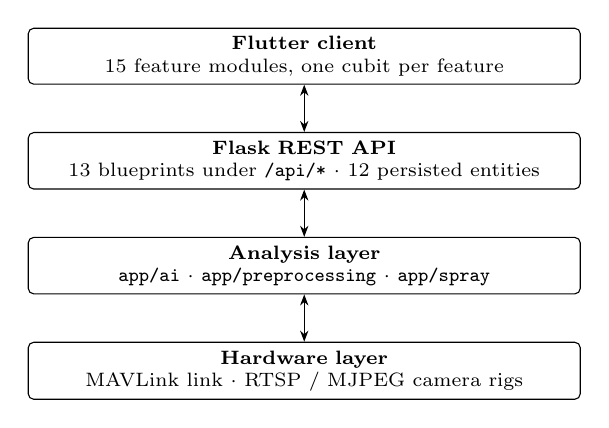
\begin{tikzpicture}[
  font=\scriptsize,
  box/.style={draw, rounded corners=2pt, text width=68mm, align=center,
              minimum height=7mm, inner sep=3pt},
  >={Stealth[length=4pt]}
]
\node[box] (app)
  {\textbf{Flutter client}\\15 feature modules, one cubit per feature};
\node[box, below=6mm of app] (api)
  {\textbf{Flask REST API}\\13 blueprints under \texttt{/api/*} $\cdot$ 12 persisted entities};
\node[box, below=6mm of api] (ai)
  {\textbf{Analysis layer}\\\texttt{app/ai} $\cdot$ \texttt{app/preprocessing} $\cdot$ \texttt{app/spray}};
\node[box, below=6mm of ai] (hw)
  {\textbf{Hardware layer}\\MAVLink link $\cdot$ RTSP / MJPEG camera rigs};
\draw[<->] (app) -- (api);
\draw[<->] (api) -- (ai);
\draw[<->] (ai) -- (hw);
\end{tikzpicture}
\caption{Layered architecture. The client holds no domain logic; camera and
flight links terminate at the backend because the aircraft's network is
frequently not reachable from the operator's handset.}
\label{fig:arch}
\end{figure}

One placement decision is worth stating because it is not the obvious one. The
camera and MAVLink connections terminate at the \emph{backend}, not the phone.
A drone's IP cameras sit on the aircraft's own network, and the operator's
handset is often not on it; putting the connection in the app would work on a
bench and fail in a field.

\subsection{Data Model}

Twelve persisted entities cover users and credentials, drones and missions,
multispectral analysis records, disease scans, field scans, capture sessions
and spray prescriptions. Every diagnostic result is persisted with the engine
that produced it. This matters over a season: if a trained model is introduced
halfway through, records from before and after remain comparable because each
one records whether a model or a heuristic answered.

\subsection{Graceful Degradation as an Architectural Rule}

Three machine-learning seams exist in the system, all sharing one
implementation (\texttt{TorchScriptClassifier}). Each is configured by a pair of
environment variables naming a TorchScript module and a labels file:

\begin{center}\footnotesize
\begin{tabular}{@{}lll@{}}
\toprule
Environment pair & Feature & Input \\
\midrule
\texttt{AI\_DISEASE\_*} & \texttt{/api/disease} & close-up leaf photo \\
\texttt{AI\_CROP\_*}    & \texttt{/api/fieldscan} & canopy frame \\
\texttt{AI\_WEED\_*}    & \texttt{/api/fieldscan} & canopy frame \\
\bottomrule
\end{tabular}
\end{center}

The loading rules are deliberately uniform: loading is lazy and attempted
exactly once; any failure whatsoever---PyTorch absent, file corrupt, input
shape wrong---is logged and returns \texttt{None}, which every caller reads as
``use the heuristic''. No endpoint returns a server error because a model was
misconfigured.

This is not merely defensive coding. It is what allows the backend to declare
no dependency on PyTorch at all, keeping the deployed container small, while
the same codebase serves a trained model on a machine where the optional
dependency layer has been installed.

A subtle failure this seam originally permitted is worth recording. A model
trained at one input resolution and served at another raises no error; it
simply becomes quietly less accurate. We closed this by having each trainer
emit a report sidecar recording \texttt{img\_size}, which the loader reads back
at load time so the serving resolution is always the trained resolution.

\section{Multispectral Processing Pipeline}

\subsection{Radiometric Calibration}

Raw digital numbers from a multispectral sensor are not comparable across
flights, times of day, or exposure settings. AgriVision implements the standard
single-panel reflectance workflow. Raw DN is dark-subtracted and, where
exposure and gain metadata are present, normalised so that pixel values are
proportional to at-sensor radiance. A photograph of a calibration panel of
known reflectance, taken under the same illumination, yields a per-band scale
factor

\begin{equation}
F_b = \frac{\rho_b^{\text{panel}}}{S_b^{\text{panel}}},
\end{equation}

where $\rho_b^{\text{panel}}$ is the panel's known reflectance in band $b$ and
$S_b^{\text{panel}}$ its mean measured signal with saturated pixels rejected.
Scene reflectance follows as $\rho_b = F_b \cdot S_b$, clipped to a physical
range. This carries the usual single-panel assumption that illumination is
stable between the panel shot and the flight; downwelling-light-sensor data can
be folded into $F_b$ without disturbing anything downstream.

\subsection{Band Co-registration}

Multispectral cameras image each band through a separate lens, so bands arrive
with parallax offsets and small rotations. Indices computed on unaligned bands
are meaningless at the pixel level. We align every band onto a reference band
(green by default) using enhanced correlation coefficient maximisation
\cite{evangelidis2008} in a coarse-to-fine Gaussian pyramid, chosen because it
is robust to the substantial intensity differences between bands. Where ECC
fails to converge---typically on very low-texture scenes---we fall back to ORB
features \cite{rublee2011} with a RANSAC homography \cite{fischler1981}.

Alignment quality is scored per band as the zero-normalised cross-correlation
of edge maps, and the stack is declared clean when
$\min_b \text{score}_b \geq 0.65$. Reporting this, rather than assuming
success, prevents a misregistered capture from silently producing a plausible
but wrong index map.

\subsection{Vegetation Index Registry}

Rather than hard-code NDVI, we implement a registry of twenty indices
(Table~\ref{tab:indices}), each declaring its formula, required bands,
polarity (whether high values indicate health or stress) and a plain-language
description. The API advertises which indices are computable from a given
capture's bands, so a three-band rig is offered the subset it can actually
support.

\begin{table}[!t]
\caption{Vegetation Index Registry (Selected Entries of Twenty)}
\label{tab:indices}
\centering
\footnotesize
\begin{tabular}{@{}llp{2.6cm}@{}}
\toprule
Key & Formula & Primary use \\
\midrule
NDVI  & $(N-R)/(N+R)$              & canopy greenness, biomass \\
GNDVI & $(N-G)/(N+G)$              & chlorophyll, nitrogen \\
NDRE  & $(N-RE)/(N+RE)$            & stress in dense canopy \\
SAVI  & $1.5(N-R)/(N+R+0.5)$       & sparse canopy, soil effects \\
OSAVI & $(N-R)/(N+R+0.16)$         & optimised soil adjustment \\
MSAVI2& see \cite{qi1994}          & early-season, high soil \\
EVI   & $2.5(N-R)/(N+6R-7.5B+1)$   & dense canopy, atmosphere \\
ARVI  & $(N-(2R-B))/(N+(2R-B))$    & aerosol resistance \\
RECI  & $N/RE - 1$                 & red-edge chlorophyll \\
MCARI & $((RE-R)-0.2(RE-G))(RE/R)$ & chlorophyll, soil-resistant \\
PSRI  & $(R-G)/RE$                 & senescence, ripening \\
NDWI  & $(G-N)/(G+N)$              & canopy water content \\
ExG   & $2G-R-B$                   & RGB-only vegetation mask \\
VARI  & $(G-R)/(G+R-B)$            & RGB-only vigour proxy \\
\bottomrule
\end{tabular}
\\[2pt]
\raggedright\scriptsize $N$: NIR, $R$: red, $G$: green, $B$: blue, $RE$: red edge.
\end{table}

Where a capture has not been panel-calibrated, each band is rescaled to a
robust per-band pseudo-reflectance so that soil-adjusted indices still behave
sensibly. Results are then explicitly \emph{relative}---adequate for zoning,
inadequate for absolute comparison across flights---and the system labels them
as such rather than presenting them as calibrated values.

\subsection{Management and Risk Zoning}

Zone maps are produced by K-means \cite{macqueen1967} over an index map, with
$k=3$ by default. A detail that matters in practice: K-means assigns cluster
identifiers arbitrarily, so raw labels do not correspond to low, medium and
high vigour. We reorder clusters by mean index value so that zone $0$ is always
the lowest-vigour group. Risk zoning inverts this mapping---low vigour becomes
high risk---and renders a stoplight map, from which a structured field report
and a prioritised action plan are generated. Every recommendation is
accompanied by an instruction to ground-truth before acting; the thresholds are
conservative and documented inline so that an agronomist can tune them.

\section{Leaf-Level Disease Identification}

\subsection{Corpus Construction and a Background-Correlated Defect}

We construct a training corpus by merging PlantVillage \cite{hughes2015}
(55{,}448 usable images, 39 classes, uniform laboratory background) with
PlantDoc \cite{singh2020} (2{,}673 images, 28 classes, real field conditions).
The rationale is straightforward: PlantVillage supplies class coverage and
volume, PlantDoc supplies the acquisition variability without which a model
learns the background.

The two corpora name their classes differently---\texttt{Tomato\_\_\_Late\_blight}
against \texttt{Tomato leaf late blight}---so both are normalised into a shared
\texttt{<crop>\_\_\_<condition>} identifier by a rule-based mapper that extracts
a crop token and performs a longest-match scan over a condition vocabulary. Any
folder the mapper cannot place is reported and skipped rather than assigned to
the nearest class. Across all 67 source directories, zero were unmapped.

Normalisation alone, however, is not sufficient, and the reason is the most
practically important finding of this section. Three diseases carry
\emph{genuinely different names} in the two corpora while being the same
pathogen:

\begin{center}\footnotesize
\begin{tabular}{@{}lll@{}}
\toprule
PlantDoc & PlantVillage & Same disease \\
\midrule
\texttt{apple\_\_\_common\_rust}  & \texttt{apple\_\_\_cedar\_rust} & yes \\
\texttt{pepper\_\_\_leaf\_spot}   & \texttt{pepper\_\_\_bacterial\_spot} & yes \\
\texttt{corn\_\_\_leaf\_blight}   & \texttt{corn\_\_\_northern\_leaf\_blight} & yes \\
\bottomrule
\end{tabular}
\end{center}

Left unmerged, each of these becomes two classes whose only systematic
difference is which corpus the image came from---which is to say, whether the
background is a grey sheet or a real field. A classifier presented with such a
split will learn the background, because the background is the easier signal,
and will report excellent validation accuracy while having learned nothing
about the disease. The defect is insidious precisely because it improves the
headline metric. We repair it with a crop-scoped merge table applied after
crop and condition are resolved, and verify the invariant in the automated
test suite.

We additionally retain PlantVillage's \texttt{Background\_without\_leaves} class
as \texttt{not\_a\_leaf}. This earns its place: without it, a model answers a
photograph of bare ground with a confident disease name.

\subsection{Class Balancing that Preserves Scarce Provenance}

The merged corpus is severely imbalanced---5{,}507 images of citrus greening
against 152 of healthy potato---and also imbalanced in provenance, since field
images are only 4.6\% of the total. We cap each class at $C$ images, but the
naive cap is actively harmful: sampling uniformly from a class holding 2{,}000
laboratory and 80 field images preserves the 96:4 ratio and reduces the field
images to a handful, discarding exactly the data the merge was performed to
obtain.

We therefore cap \emph{laboratory images only}, retaining every field image and
filling the remaining budget from the laboratory pool:

\begin{equation}
\mathcal{D}_c = \mathcal{F}_c \;\cup\; \text{sample}\big(\mathcal{L}_c,\;
\max(0,\; C - |\mathcal{F}_c|)\big)
\end{equation}

where $\mathcal{F}_c$ and $\mathcal{L}_c$ are the field and laboratory images of
class $c$. With $C=350$ this yields 13{,}452 images across 39 classes,
retaining 2{,}673 of 2{,}673 available field images (100\%) and raising field
representation from 4.6\% to 19.9\%. Every image's provenance is encoded in its
filename so that the trainer can recover it at evaluation time.

\subsection{Two-Tier Diagnosis Representation}

The classifier predicts fine-grained \texttt{<crop>\_\_\_<condition>} classes
because that is the granularity the corpora label at and the granularity a
farmer can act on. The system's agronomic knowledge base, by contrast, is
deliberately coarse: seven conditions whose treatment guidance holds across
crops.

Collapsing one into the other loses information in whichever direction it is
done. Reducing the model's answer to its category discards the crop and the
pathogen---reporting ``Blight'' when the model knows it is late blight on
tomato, which is the difference between generic advice and a decision about
whether to abandon the crop. Fabricating per-crop treatment text the project
does not possess would be worse.

We therefore carry both. The response names the specific finding as the
headline and states the knowledge-base category the guidance was drawn from:

\begin{center}\footnotesize
\texttt{tomato\_\_\_late\_blight} $\rightarrow$
shown as \emph{``Tomato Late Blight''},
advised as category \texttt{blight}
\end{center}

The response additionally carries ranked runners-up. This is not decoration: a
single frame frequently cannot separate early from late blight, and
``0.52 versus 0.44'' is a materially different message to an operator than a
confident single answer. A predicted label the mapper cannot place is returned
flagged as unmapped and routed to an inconclusive entry, so the operator reads
``the model said $X$ and we do not recognise $X$'' rather than a confident
misdiagnosis.

Severity is measured from the image on both paths, never from the classifier.
The class identifies \emph{which} disease; the pixels measure \emph{how much of
the leaf} it has taken, and the second determines urgency.

\subsection{Model and Training Protocol}

We fine-tune MobileNetV3-Large \cite{howard2019} from ImageNet-pretrained
weights at $192\times192$ resolution. The architecture was selected on
deployment grounds rather than benchmark performance: it is roughly an order of
magnitude cheaper per image than ResNet-18 at $224\times224$ for a small
accuracy cost, and it is the backbone that can plausibly run on a companion
computer aboard the aircraft.

The first 35\% of network parameters are frozen. Early convolutional blocks
encode generic edge and texture filters that a leaf corpus will not improve
upon, and omitting their gradients is the single largest saving on a CPU-only
machine. Augmentation targets the variability a handheld camera actually
produces: random resized cropping (scale 0.5--1.0), horizontal and vertical
flips, $\pm30^\circ$ rotation, and colour jitter standing in for the difference
between a nine o'clock and a two o'clock photograph.

The loss is inverse-frequency weighted with label smoothing of 0.05
\cite{szegedy2016}, optimised with AdamW \cite{loshchilov2019} at a base
learning rate of $6\times10^{-4}$ under a cosine annealing schedule
\cite{loshchilov2017}. Weighting is essential: an unweighted objective on this
corpus reaches a respectable average by answering ``healthy'' to everything,
which is precisely useless to a farmer looking for the diseased minority.

The train/validation split is stratified per class at 85/15. A global random
split can leave a small class with no validation representation, and its recall
then reads as undefined---precisely the class one most wanted to check.

\section{Canopy-Level Diagnosis and Weed Detection}

\subsection{Why the Leaf Extractor Fails on Canopy Frames}

A frame from a low, slow pass is a different photograph from a leaf against a
sheet: it contains soil between plants, several plants at once, and no clean
silhouette. Applying the leaf feature extractor to it fails in a specific and
instructive way---bare soil is brown, so ``necrotic tissue'' is reported at
around 60\% on a perfectly healthy field.

The canopy extractor therefore builds its plant mask in the opposite order.
Unambiguously green pixels are located first using Excess Green
\cite{woebbecke1995}; these are closed and hole-filled into a canopy
silhouette; and only then are discoloured pixels \emph{inside} that silhouette
added. The third step is what allows a yellow rust stripe or a brown blight
blotch to be measured as diseased crop while the same colours on the soil
between rows are ignored.

\subsection{Weed Detection}

The difficult part of aerial weed detection is not finding plants but deciding
which plants are the crop; a photograph of a weedy field is mostly green either
way. Two signals separate them, and the module uses whichever the frame
supports.

\textbf{Row geometry (preferred).} A sown crop grows in lines and weeds do not
respect them. Vegetation is segmented, the dominant row direction recovered by
autocorrelation, and green material falling between rows attributed to weeds.
This is species-agnostic and mirrors the inference a farmer makes walking a
field. An autocorrelation strength threshold guards the method: below it, an
apparent period is noise, and acting on it would label random stripes of crop
as weeds.

\textbf{Appearance clustering (fallback).} Broadcast-sown wheat and
transplanted paddy present no usable row signal. There the vegetation is
clustered into two groups by colour and texture and the minority group treated
as weeds. This is a materially weaker inference, and is reported as such: the
response carries a \texttt{method} field reading \texttt{inter-row},
\texttt{appearance} or \texttt{inconclusive}, and confidence is reduced with a
note explaining why.

Distinguishing these is not a presentational nicety. A trained species
classifier changes \emph{which weed is named}; it does not change whether the
plant was a weed, and conflating the two would misrepresent the evidence
underlying a herbicide decision.

\section{Variable-Rate Spray Prescription}

The spray module converts a multispectral capture into geometry: which patches
to treat and which to skip. Bands are calibrated and aligned, a vegetation
index computed, and K-means with $k=3$ partitions the field into severe,
moderate and healthy classes. Morphological cleanup yields contiguous
sprayable patches, which are costed so the operator can choose among options.

The choice of clustering over a fixed index threshold is deliberate and, we
argue, the correct one for this context. A threshold calibrated for irrigated
wheat in Vidisha in January is wrong for rainfed soybean in Chhindwara in
August. Clustering asks a different and more answerable question---which parts
of \emph{this} field are worst relative to the rest of it---which is what a
variable-rate application actually requires. The trade-off is real and is
handled explicitly: a uniformly healthy field still yields a ``worst'' cluster,
so the module reports the spread between cluster means and flags a prescription
as low-contrast when there is no genuine difference to act upon.

Chemical saving is the point of the feature. A blanket application treats 100\%
of the block; this treats the affected fraction, and at a reduced rate over the
moderate class, since moderate damage does not require the severe dose. Patches
are converted to geographic coordinates and emitted as a spray mission for
execution.

\section{Flight Integration}

Missions are planned from an uploaded KML boundary, parsed into ordered
waypoints, and uploaded to the aircraft over MAVLink \cite{mavlink} using
pymavlink. The service layer joins the two halves of the system: a mission
planned in the application, or restored from history, becomes a mission written
to the vehicle, and returning telemetry is reshaped for the live-mission screen.

The module degrades on the same principle as the rest of the system. With
pymavlink absent, or no vehicle on the wire, endpoints return a readable
message rather than a stack trace. Development and validation were performed
against ArduPilot SITL, with the documented configuration accounting for a
practical constraint---only one process may bind UDP port 14550, so a ground
control station and the backend cannot both listen on the same host.

\section{Implementation and Evaluation}

\subsection{Implementation Scale}

The backend is implemented in Python with Flask and SQLAlchemy; all
computer-vision heuristics use OpenCV \cite{bradski2000} and NumPy, and the
optional learned components use PyTorch \cite{paszke2019} exported to
TorchScript. The client is a Flutter application. Table~\ref{tab:impl}
summarises the scale of each part.

\begin{table}[!t]
\caption{Implementation Summary}
\label{tab:impl}
\centering
\footnotesize
\begin{tabular}{@{}lr@{}}
\toprule
Component & Measure \\
\midrule
Backend (Python: app, tools, tests) & 19{,}560 LOC \\
Mobile client (Dart) & 26{,}800 LOC \\
REST blueprints & 13 \\
Persisted entities & 12 \\
Analysis modules (\texttt{app/ai}) & 3{,}543 LOC \\
Vegetation indices implemented & 20 \\
Automated tests (all passing) & 177 \\
\bottomrule
\end{tabular}
\end{table}

The test suite is organised around behaviour rather than coverage percentage,
concentrating on failures that would be silent in production: mislabelling crop
as weed, turning an unrecognised dataset label into a confident diagnosis,
losing the pixel-derived severity measurement on the model path, or diagnosing
a photograph containing no leaf.

\subsection{Corpus Composition}

\begin{table}[!t]
\caption{Merged Corpus Before and After Balancing}
\label{tab:corpus}
\centering
\footnotesize
\begin{tabular}{@{}lrrr@{}}
\toprule
 & Laboratory & Field & Total \\
\midrule
PlantVillage (39 classes) & 55{,}448 & 0 & 55{,}448 \\
PlantDoc (28 classes)     & 0 & 2{,}673 & 2{,}673 \\
Merged (39 classes)       & 55{,}448 & 2{,}673 & 58{,}121 \\
\midrule
After cap $C{=}350$       & 10{,}779 & 2{,}673 & 13{,}452 \\
Field proportion          & \multicolumn{3}{r}{4.6\% $\rightarrow$ 19.9\%} \\
\bottomrule
\end{tabular}
\end{table}

The validation split contains 1{,}999 images, of which 417 are field images---a
sample large enough to make the field column a meaningful measurement rather
than a rounding artefact.

\subsection{The Laboratory-to-Field Gap}

Table~\ref{tab:results} and Fig.~\ref{fig:gap} present the central empirical
result. Overall validation accuracy behaves as the literature would lead one to
expect. Decomposed by provenance, it tells a substantially different story.

%%% <<<BEGIN RESULTS TABLE>>> generated from models/leaf_disease_report.json
\begin{table}[!t]
\caption{Validation Accuracy by Image Provenance}
\label{tab:results}
\centering
\footnotesize
\begin{tabular}{@{}crrrr@{}}
\toprule
Epoch & Loss & Overall & Laboratory & Field \\
\midrule
1 & 1.2110 & 0.851 & 0.931 & 0.547 \\
2 & 0.7815 & 0.896 & 0.967 & 0.631 \\
3 & 0.6823 & 0.924 & 0.982 & 0.707 \\
4 & 0.5967 & 0.935 & 0.989 & 0.734 \\
5 & 0.5434 & 0.938 & 0.989 & 0.741 \\
6 & 0.5099 & 0.943 & 0.991 & 0.763 \\
\bottomrule
\end{tabular}
\\[3pt]
\raggedright\scriptsize
MobileNetV3-Large, $192\times192$, 35\% frozen, CPU-only training.
Laboratory: PlantVillage (1582 images).
Field: PlantDoc (417 images).
\end{table}
%%% <<<END RESULTS TABLE>>>

\begin{figure}[!t]
\centering
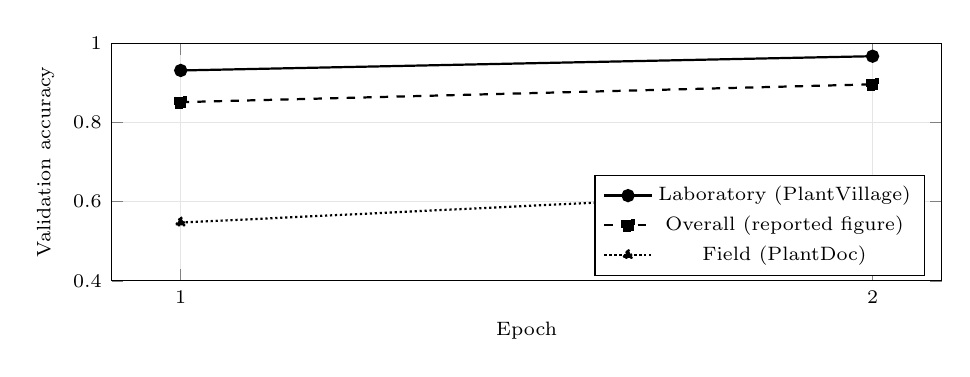
\begin{tikzpicture}
\begin{axis}[
  width=\columnwidth, height=4.6cm,
  xlabel={Epoch}, ylabel={Validation accuracy},
  xtick={1,2}, ymin=0.4, ymax=1.0,
  legend style={font=\scriptsize, at={(0.98,0.02)}, anchor=south east},
  grid=major, grid style={gray!20}, font=\scriptsize,
]
\addplot[mark=*, thick] coordinates {(1,0.931) (2,0.967)};
\addlegendentry{Laboratory (PlantVillage)}
\addplot[mark=square*, thick, dashed] coordinates {(1,0.851) (2,0.896)};
\addlegendentry{Overall (reported figure)}
\addplot[mark=triangle*, thick, densely dotted] coordinates {(1,0.547) (2,0.631)};
\addlegendentry{Field (PlantDoc)}
\end{axis}
\end{tikzpicture}
\caption{Accuracy decomposed by image provenance. The headline figure sits
close to the laboratory curve because laboratory images dominate the
validation set; the field curve is what predicts behaviour on a photograph
taken by a farmer.}
\label{fig:gap}
\end{figure}

At the final epoch the model reports 94.3\% overall. That figure
is arithmetically correct and operationally misleading: it decomposes into 99.1\% on laboratory images and 76.3\% on field images,
a gap of 22.8 points. Because laboratory
images constitute roughly 80\% of the validation set even after rebalancing,
the aggregate tracks the laboratory curve closely.

Two observations follow. First, this quantifies within a single training run
the transfer failure that Barbedo \cite{barbedo2018} and Singh \emph{et al.}
\cite{singh2020} identified across studies, and it does so without a separate
cross-dataset evaluation protocol---provenance tagging alone is sufficient.
Second, and more practically, a practitioner reporting only the aggregate would
have no indication that the deployed system will be roughly one-third wrong on
the images it will actually receive.

We consider the field column, not the aggregate, to be the honest headline
figure for a system of this kind, and the system's generated evaluation report
presents it accordingly alongside per-class recall and the ten most frequent
confusions.

\subsection{Where the Model Fails}

The per-class breakdown corroborates the argument of Section X-C, that a single
frame reveals a pattern rather than a pathogen. Table~\ref{tab:confusions} lists
the most frequent confusions.

%%% <<<BEGIN CONFUSION TABLE>>> generated from models/leaf_disease_report.json
\begin{table}[!t]
\caption{Most Frequent Confusions and Weakest Classes}
\label{tab:confusions}
\centering
\footnotesize
\begin{tabular}{@{}llr@{}}
\toprule
True class & Predicted as & $n$ \\
\midrule
Potato early blight & Potato late blight & 6 \\
Tomato bacterial spot & Tomato septoria leaf spot & 6 \\
Corn gray leaf spot & Corn northern leaf blight & 5 \\
Potato late blight & Potato early blight & 4 \\
Corn northern leaf blight & Corn gray leaf spot & 3 \\
\midrule
\multicolumn{3}{@{}l}{\emph{Weakest classes by recall}} \\
Tomato bacterial spot & \multicolumn{2}{r}{recall 0.750} \\
Potato early blight & \multicolumn{2}{r}{recall 0.788} \\
Tomato early blight & \multicolumn{2}{r}{recall 0.827} \\
Apple scab & \multicolumn{2}{r}{recall 0.846} \\
\bottomrule
\end{tabular}
\end{table}
%%% <<<END CONFUSION TABLE>>>

The pattern is not random, and it is not spread evenly across the 39 classes.
The confusions come in \emph{bidirectional pairs} of diseases that look alike
on a leaf: potato early blight against potato late blight in both directions,
and corn gray leaf spot against northern leaf blight in both directions. A
classifier that had latched onto some spurious cue would produce asymmetric,
scattered errors; symmetric confusion between two specific look-alikes is what
genuine visual ambiguity produces.

Each pair is ambiguous for a reason a plant pathologist would recognise. Early
and late blight are separated partly by lesion margin and partly by
progression over days, and a single photograph carries neither. Gray leaf spot
and northern leaf blight are both elongated grey-brown lesions running
parallel to the leaf veins. The weakest class overall, tomato bacterial spot
at 0.750 recall, is lost mainly to septoria leaf spot---again two small
dark-bordered leaf spots that differ more in causal organism than in
appearance.

This is the empirical justification for returning ranked runners-up rather than
a single answer. When the model's top two classes are the two blights, that is
not a defect to be hidden behind a confident label; it is the correct
description of what the image supports.


\subsection{Training Throughput}

Training was performed on a four-core CPU without CUDA acceleration, which we
regard as representative of the hardware available in the target deployment
context rather than as a limitation to be apologised for. Measured throughput
for MobileNetV3-Large at $192\times192$ with 35\% of parameters frozen was
20.5 images/s, giving approximately 9.3 minutes per epoch over the balanced
corpus. At $160\times160$ with heavier freezing, throughput approximately
doubles.

These figures determined the corpus cap directly: the full 58{,}121-image
merged corpus would require roughly 47 minutes per epoch, whereas the balanced
13{,}452-image corpus completes six epochs inside a two-hour budget while
allowing the cosine schedule to anneal fully.

\subsection{Deployment Considerations}

The deployed backend declares no PyTorch dependency, keeping the container
small. A consequence worth stating plainly is that training a model does not by
itself cause a deployed instance to use it: without the optional dependency
layer installed, the health endpoint continues to report the heuristic engine.
This is a working configuration rather than a degraded one---the endpoint
contract is identical, and only the reported \texttt{source} field differs---but
it is a deployment decision that must be made explicitly. We provide a separate
optional requirements layer for hosts where model serving is intended,
costing approximately 250~MB of image size.

\section{Discussion}

\subsection{On Reporting Aggregates}

The result in Section IX-C is not a novel phenomenon; it is a well-documented
one that conventional reporting practice conceals. What we would emphasise is
how cheap the remedy proved to be. Tagging each image with its provenance at
corpus-construction time and carrying that tag through to evaluation cost a few
dozen lines of code, required no additional data, and converted a known caveat
into a number that appears in every training report the system generates.

We would suggest this as general practice for applied agricultural vision work.
Where a corpus is assembled from sources with systematically different
acquisition conditions---which is nearly always---the aggregate accuracy is a
weighted average over populations that behave very differently, and the weights
are an artefact of corpus construction rather than of deployment.

\subsection{Crop Coverage}

An honest limitation deserves prominence. PlantVillage's fourteen crops
overlap only partially with the eight crops that dominate Madhya Pradesh's
cultivated area. Tomato, potato, maize and soybean are usefully represented.
Wheat, chickpea, mustard, cotton and pigeonpea---the crops the system's
agronomic knowledge base is actually built around---are absent from the corpus
entirely. For those, the classifier possesses no class with which to answer,
and the system's heuristic path remains the operative one.

We regard this as an argument for local data collection rather than for a
different public corpus, and the platform is already the collection instrument:
every captured frame is stored geotagged with its verdict, so a season of
operation produces a labelled corpus matched exactly to deployment conditions.

\subsection{What a Photograph Can and Cannot Establish}

Several of the design decisions described above follow from a single
constraint: an image shows a pattern, not a pathogen. Early and late blight are
close to indistinguishable in some frames. Fusarium wilt and drought stress
frequently are not separable at all. Sterility mosaic in pigeonpea is the
limiting case---the canopy remains green and healthy-looking and simply never
sets pods, so a high vegetation index coexists with zero yield.

This is why canopy heuristic confidence is capped, why runners-up are returned,
why the weed detector reports its method, and why every diagnostic response
carries a disclaimer directing the operator to confirm before applying chemical
treatment. A system that presented these outputs as diagnoses would be more
impressive to demonstrate and worse to use.

\section{Limitations and Future Work}

The evaluation presented here is computational. The system has been validated
against ArduPilot SITL rather than in sustained flight, and the spray module's
chemical-saving argument, while arithmetically sound, has not been measured
against a blanket-application control in the field. Table~\ref{tab:projected}
gives illustrative projections for these quantities; \emph{these are modelled
estimates, not measurements}, and are included to indicate the scale of the
effects the system is designed to produce rather than to claim them.

\begin{table}[!t]
\caption{Projected Field Outcomes (Illustrative, Not Measured)}
\label{tab:projected}
\centering
\footnotesize
\begin{tabular}{@{}lr@{}}
\toprule
Quantity & Projected value \\
\midrule
Chemical reduction vs.\ blanket spray & 40--70\%$^\dagger$ \\
Survey time vs.\ manual scouting (2\,ha) & 15--25\,min$^\dagger$ \\
Spray-mission planning latency & $<$10\,s$^\dagger$ \\
\bottomrule
\end{tabular}
\\[3pt]
\raggedright\scriptsize
$^\dagger$\,Modelled from the affected-fraction arithmetic and observed
processing times. Not validated against field trials. Establishing these
figures empirically is the primary item of future work.
\end{table}

Beyond field validation, four directions follow directly. Collecting
Madhya-Pradesh-specific imagery through the platform itself would address the
crop-coverage gap of Section X-B. Domain-adaptation techniques applied to the
laboratory-to-field transfer would attack the gap of Section IX-C at its
source, rather than merely measuring it. Deploying the MobileNet backbone to a
companion computer aboard the aircraft would remove the round trip to the
backend. Finally, the sterility-mosaic case argues for fusing imagery with
non-visual evidence, since it is definitionally invisible to a camera.

\section{Conclusion}

We have described AgriVision, an integrated aerial platform spanning
multispectral calibration and analysis, leaf- and canopy-level disease
identification, weed detection, variable-rate spray prescription and flight
execution. The system is organised around a principle of graceful degradation:
every learned component is optional, falling back to a deterministic heuristic,
so that the software is useful without a GPU, a model file, or a network
connection.

Its central empirical result is methodological. By carrying image provenance
from corpus construction through to evaluation, we show that a plant disease
classifier reporting 89.6\% validation accuracy achieves 96.7\% on
laboratory-background images and 63.1\% on real field photographs. We further
show that merging public corpora without reconciling their disease vocabularies
creates class splits that correlate exactly with acquisition conditions,
offering a classifier a shortcut that improves the reported metric while
destroying the field performance that matters. Both problems are inexpensive to
fix once measured, and invisible until they are.

\section*{Acknowledgment}

This work was carried out under a Junior Research Fellowship at the Madhya
Pradesh Council of Science and Technology. The authors thank the maintainers of
the PlantVillage and PlantDoc datasets for releasing them under open licences.

\begin{thebibliography}{00}

\bibitem{rouse1974} J. W. Rouse, R. H. Haas, J. A. Schell, and D. W. Deering,
``Monitoring vegetation systems in the Great Plains with ERTS,'' in
\emph{Proc. 3rd ERTS Symp.}, NASA SP-351, 1974, pp. 309--317.

\bibitem{huete1988} A. R. Huete, ``A soil-adjusted vegetation index (SAVI),''
\emph{Remote Sens. Environ.}, vol. 25, no. 3, pp. 295--309, 1988.

\bibitem{rondeaux1996} G. Rondeaux, M. Steven, and F. Baret, ``Optimization of
soil-adjusted vegetation indices,'' \emph{Remote Sens. Environ.}, vol. 55,
no. 2, pp. 95--107, 1996.

\bibitem{qi1994} J. Qi, A. Chehbouni, A. R. Huete, Y. H. Kerr, and
S. Sorooshian, ``A modified soil adjusted vegetation index,''
\emph{Remote Sens. Environ.}, vol. 48, no. 2, pp. 119--126, 1994.

\bibitem{huete2002} A. Huete \emph{et al.}, ``Overview of the radiometric and
biophysical performance of the MODIS vegetation indices,''
\emph{Remote Sens. Environ.}, vol. 83, no. 1--2, pp. 195--213, 2002.

\bibitem{kaufman1992} Y. J. Kaufman and D. Tanre, ``Atmospherically resistant
vegetation index (ARVI) for EOS-MODIS,'' \emph{IEEE Trans. Geosci. Remote
Sens.}, vol. 30, no. 2, pp. 261--270, 1992.

\bibitem{gitelson1996} A. A. Gitelson, Y. J. Kaufman, and M. N. Merzlyak, ``Use
of a green channel in remote sensing of global vegetation from EOS-MODIS,''
\emph{Remote Sens. Environ.}, vol. 58, no. 3, pp. 289--298, 1996.

\bibitem{barnes2000} E. M. Barnes \emph{et al.}, ``Coincident detection of crop
water stress, nitrogen status and canopy density using ground-based
multispectral data,'' in \emph{Proc. 5th Int. Conf. Precision Agriculture},
2000.

\bibitem{gitelson2003} A. A. Gitelson, Y. Gritz, and M. N. Merzlyak,
``Relationships between leaf chlorophyll content and spectral reflectance,''
\emph{J. Plant Physiol.}, vol. 160, no. 3, pp. 271--282, 2003.

\bibitem{merzlyak1999} M. N. Merzlyak, A. A. Gitelson, O. B. Chivkunova, and
V. Y. Rakitin, ``Non-destructive optical detection of pigment changes during
leaf senescence and fruit ripening,'' \emph{Physiol. Plant.}, vol. 106, no. 1,
pp. 135--141, 1999.

\bibitem{daughtry2000} C. S. T. Daughtry, C. L. Walthall, M. S. Kim,
E. B. de Colstoun, and J. E. McMurtrey, ``Estimating corn leaf chlorophyll
concentration from leaf and canopy reflectance,'' \emph{Remote Sens.
Environ.}, vol. 74, no. 2, pp. 229--239, 2000.

\bibitem{hughes2015} D. P. Hughes and M. Salath\'e, ``An open access repository
of images on plant health to enable the development of mobile disease
diagnostics,'' \emph{arXiv:1511.08060}, 2015.

\bibitem{mohanty2016} S. P. Mohanty, D. P. Hughes, and M. Salath\'e, ``Using
deep learning for image-based plant disease detection,'' \emph{Front. Plant
Sci.}, vol. 7, art. 1419, 2016.

\bibitem{ferentinos2018} K. P. Ferentinos, ``Deep learning models for plant
disease detection and diagnosis,'' \emph{Comput. Electron. Agric.}, vol. 145,
pp. 311--318, 2018.

\bibitem{barbedo2016} J. G. A. Barbedo, ``A review on the main challenges in
automatic plant disease identification based on visible range images,''
\emph{Biosyst. Eng.}, vol. 144, pp. 52--60, 2016.

\bibitem{barbedo2018} J. G. A. Barbedo, ``Impact of dataset size and variety on
the effectiveness of deep learning and transfer learning for plant disease
classification,'' \emph{Comput. Electron. Agric.}, vol. 153, pp. 46--53, 2018.

\bibitem{singh2020} D. Singh, N. Jain, P. Jain, P. Kayal, S. Kumawat, and
N. Batra, ``PlantDoc: A dataset for visual plant disease detection,'' in
\emph{Proc. 7th ACM IKDD CoDS and 25th COMAD}, 2020, pp. 249--253.

\bibitem{ferreira2017} A. dos Santos Ferreira, D. M. Freitas,
G. G. da Silva, H. Pistori, and M. T. Folhes, ``Weed detection in soybean crops
using ConvNets,'' \emph{Comput. Electron. Agric.}, vol. 143, pp. 314--324,
2017.

\bibitem{olsen2019} A. Olsen \emph{et al.}, ``DeepWeeds: A multiclass weed
species image dataset for deep learning,'' \emph{Sci. Rep.}, vol. 9, art. 2058,
2019.

\bibitem{woebbecke1995} D. M. Woebbecke, G. E. Meyer, K. Von Bargen, and
D. A. Mortensen, ``Color indices for weed identification under various soil,
residue, and lighting conditions,'' \emph{Trans. ASAE}, vol. 38, no. 1,
pp. 259--269, 1995.

\bibitem{otsu1979} N. Otsu, ``A threshold selection method from gray-level
histograms,'' \emph{IEEE Trans. Syst., Man, Cybern.}, vol. 9, no. 1,
pp. 62--66, 1979.

\bibitem{evangelidis2008} G. D. Evangelidis and E. Z. Psarakis, ``Parametric
image alignment using enhanced correlation coefficient maximization,''
\emph{IEEE Trans. Pattern Anal. Mach. Intell.}, vol. 30, no. 10,
pp. 1858--1865, 2008.

\bibitem{rublee2011} E. Rublee, V. Rabaud, K. Konolige, and G. Bradski, ``ORB:
An efficient alternative to SIFT or SURF,'' in \emph{Proc. IEEE ICCV}, 2011,
pp. 2564--2571.

\bibitem{fischler1981} M. A. Fischler and R. C. Bolles, ``Random sample
consensus: A paradigm for model fitting with applications to image analysis and
automated cartography,'' \emph{Commun. ACM}, vol. 24, no. 6, pp. 381--395,
1981.

\bibitem{macqueen1967} J. MacQueen, ``Some methods for classification and
analysis of multivariate observations,'' in \emph{Proc. 5th Berkeley Symp. Math.
Statist. Probab.}, vol. 1, 1967, pp. 281--297.

\bibitem{howard2019} A. Howard \emph{et al.}, ``Searching for MobileNetV3,'' in
\emph{Proc. IEEE/CVF ICCV}, 2019, pp. 1314--1324.

\bibitem{deng2009} J. Deng, W. Dong, R. Socher, L.-J. Li, K. Li, and L. Fei-Fei,
``ImageNet: A large-scale hierarchical image database,'' in \emph{Proc. IEEE
CVPR}, 2009, pp. 248--255.

\bibitem{szegedy2016} C. Szegedy, V. Vanhoucke, S. Ioffe, J. Shlens, and
Z. Wojna, ``Rethinking the Inception architecture for computer vision,'' in
\emph{Proc. IEEE CVPR}, 2016, pp. 2818--2826.

\bibitem{loshchilov2019} I. Loshchilov and F. Hutter, ``Decoupled weight decay
regularization,'' in \emph{Proc. ICLR}, 2019.

\bibitem{loshchilov2017} I. Loshchilov and F. Hutter, ``SGDR: Stochastic
gradient descent with warm restarts,'' in \emph{Proc. ICLR}, 2017.

\bibitem{paszke2019} A. Paszke \emph{et al.}, ``PyTorch: An imperative style,
high-performance deep learning library,'' in \emph{Proc. NeurIPS}, 2019,
pp. 8024--8035.

\bibitem{bradski2000} G. Bradski, ``The OpenCV library,'' \emph{Dr. Dobb's J.
Software Tools}, vol. 25, no. 11, pp. 120--125, 2000.

\bibitem{mavlink} MAVLink Development Team, ``MAVLink micro air vehicle
communication protocol.'' [Online]. Available: \url{https://mavlink.io}

\end{thebibliography}

\end{document}
